\documentclass[hyperref={colorlinks = true,
                         urlcolor = blue,
                         linkcolor = blue}]{beamer}
\RequirePackage{amsmath,amssymb,amsthm}
\RequirePackage{bm}
\RequirePackage{bbm}
\RequirePackage{tikz}
\RequirePackage{dot2texi}
\usetikzlibrary{positioning,calc}
\usetikzlibrary{shapes,arrows}
\newcommand{\E}{\mathbb{E}}

% beamer tweaks
\usefonttheme[onlymath]{serif} % make beamer math look like article math
\setbeamertemplate{navigation symbols}{} % ditch beamer nav icons
\definecolor{dark-gray}{gray}{0.2}
\setbeamercolor{title}{fg=dark-gray}
\setbeamercolor{frametitle}{fg=dark-gray}
\setbeamertemplate{frametitle}[default][center]
\setbeamerfont{institute}{size=\fontsize{7pt}{8pt}}
\setbeamerfont{title}{series=\bfseries}
\setbeamertemplate{itemize items}[default]
\setbeamertemplate{enumerate items}[default]


\title{A Genealogical Look at Shared Ancestry\\on the X Chromosome}
\author{Vince Buffalo\inst{1}, Stephen M. Mount\inst{2}, Graham Coop\inst{1}}
\institute[]{
  \inst{1}%
    Department of Evolution and Ecology,\\Center for Population Biology\\
    UC Davis
  \and
  \inst{2}%
    Department of Cell Biology and Molecular Genetics,\\Center for Bioinformatics and Computational Biology\\
    University of Maryland
}



\begin{document}

\begin{frame}
  \titlepage
  \begin{tikzpicture}[remember picture,overlay,slidetitle/.style={text width=0.95*\textwidth,align=center},
    slideauthor/.style={text width=0.95*\textwidth,align=center}]
    \node[at=(current page.south west),anchor=south west,inner sep=8pt] {
      
\includegraphics[width=0.16\textwidth]{fig/coop.png}};
    \node[at=(current page.south east),anchor=south east,inner sep=8pt] {
      
\includegraphics[width=0.2\textwidth]{fig/ucd}};
  \end{tikzpicture}
\end{frame}

\begin{frame}
  \frametitle{bioRxiv preprint and blog post}
  \begin{columns}[c]
    \begin{column}{.6\textwidth}

      Details of this work are in our bioRxiv preprint: \url{http://bit.ly/x-preprint} \\[4em]

      We've also written a blog post for a general audience about X chromosome
      ancestry and genetic genealogy: \url{http://bit.ly/x-ancestry}

    \end{column}
    \begin{column}{.4\textwidth}
    \end{column}
    \begin{tikzpicture}[remember picture,overlay]
      \fboxrule=0.1pt
      \fboxsep=0mm
    \node[at=(current page.south east),anchor=south east,inner sep=8pt] {
      \fcolorbox{gray}{gray}{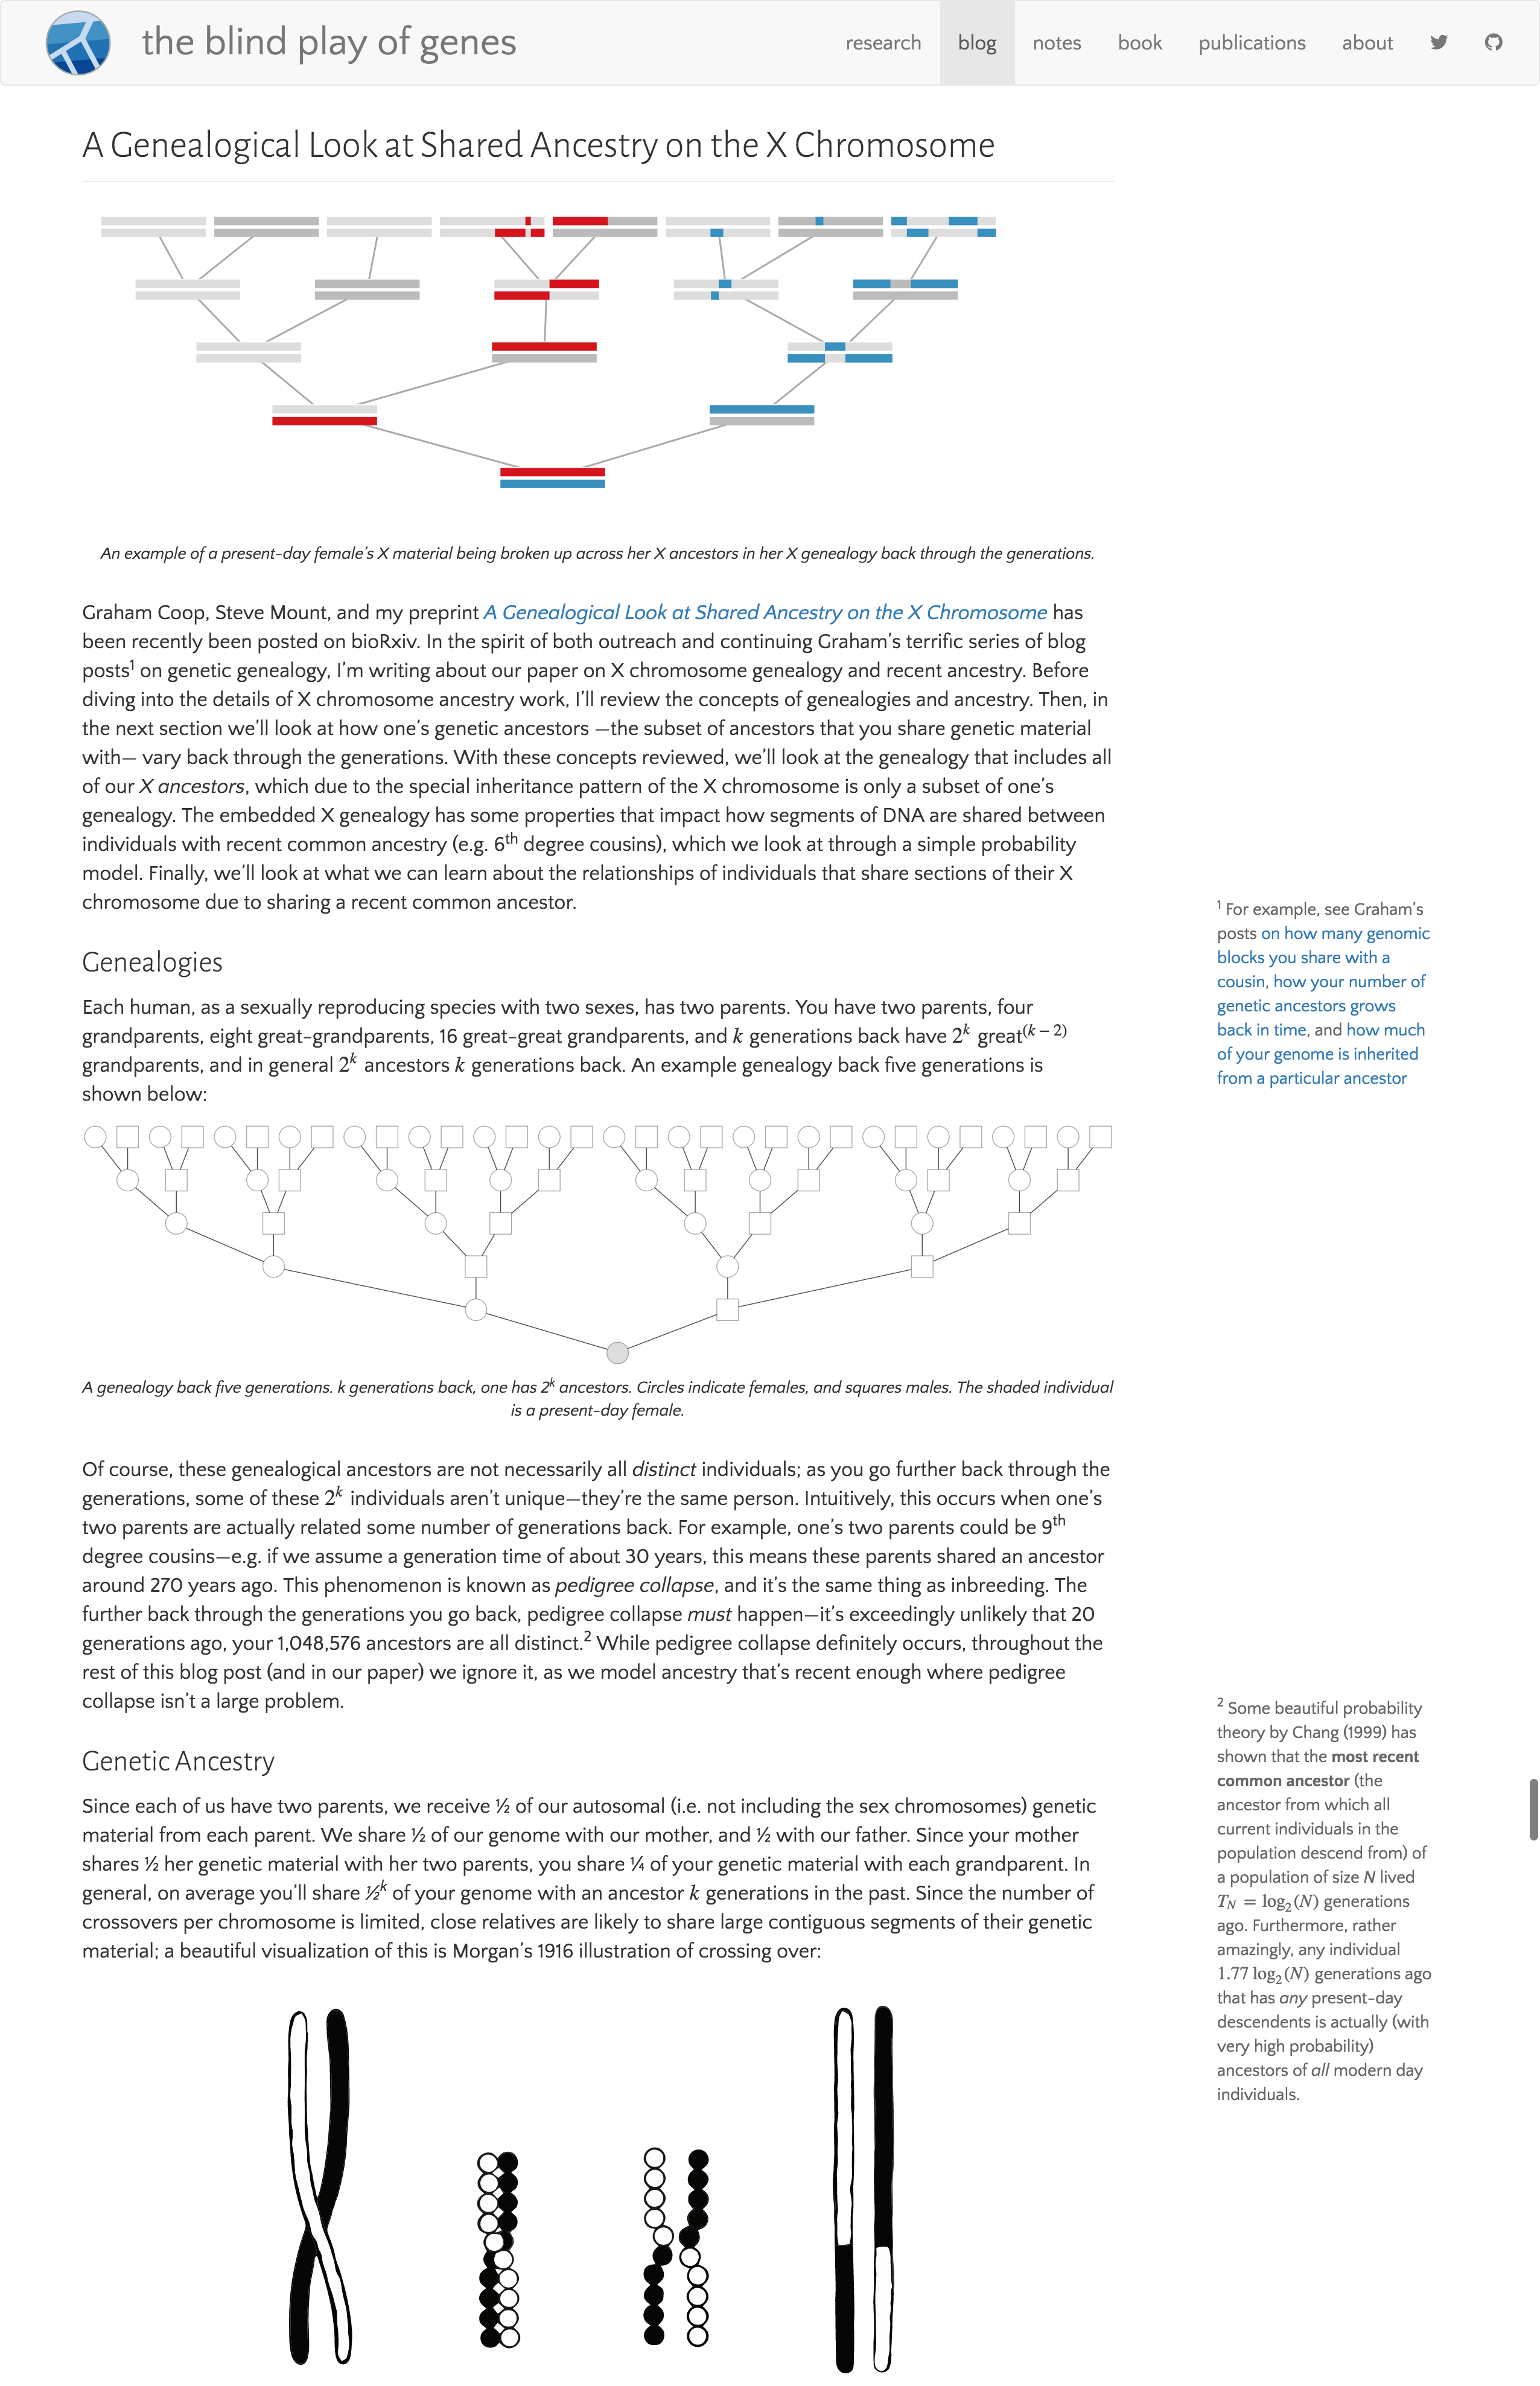
\includegraphics[height=0.8\textheight]{fig/blog-post-crop.png}}};
    \end{tikzpicture}
 
  \end{columns}
\end{frame}

\begin{frame}
  \frametitle{Genealogies}

  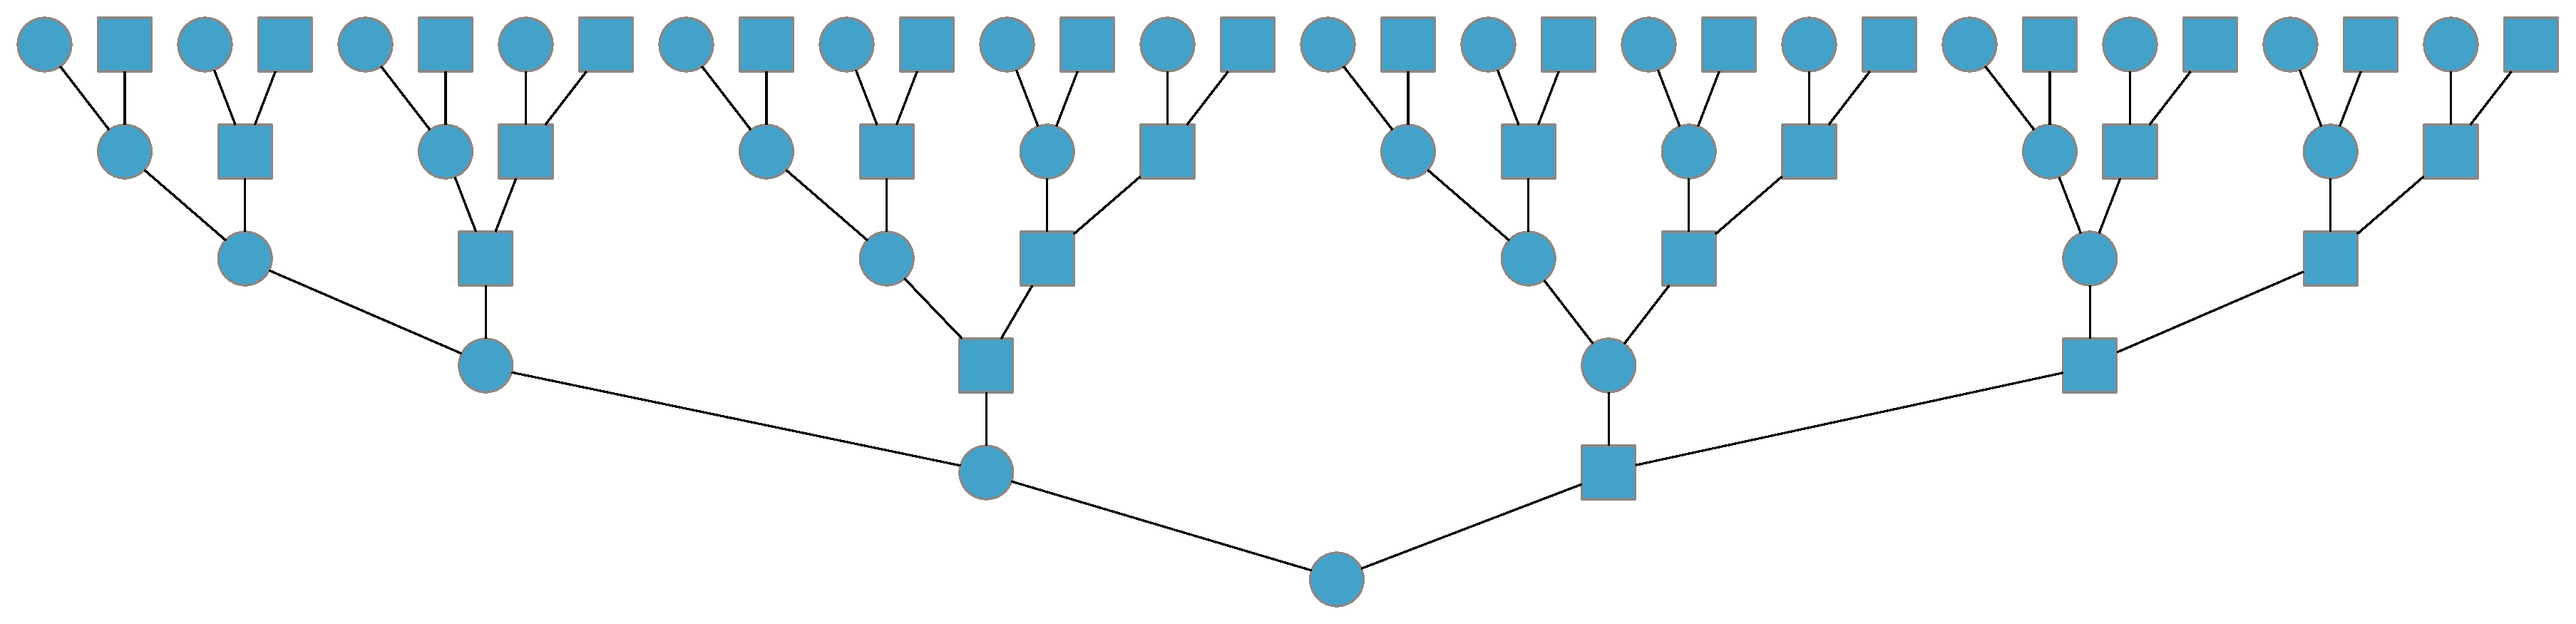
\includegraphics[width=\textwidth]{fig/genealogy}

  One's \textbf{genealogy} contains all biparental relationships back in time
  of a present-day individual.\\[1em]

  These include your two parents, four grandparents, eight great-grandparents,
  \ldots, your $2^k$ $\text{great}^{k-2}$ grandparents, and in general the
  $2^k$ ancestors $k$ generations back. These are one's \textbf{genealogical}
  ancestors.\\[2em]

\end{frame}

\begin{frame}
  \frametitle{X Genealogies}
  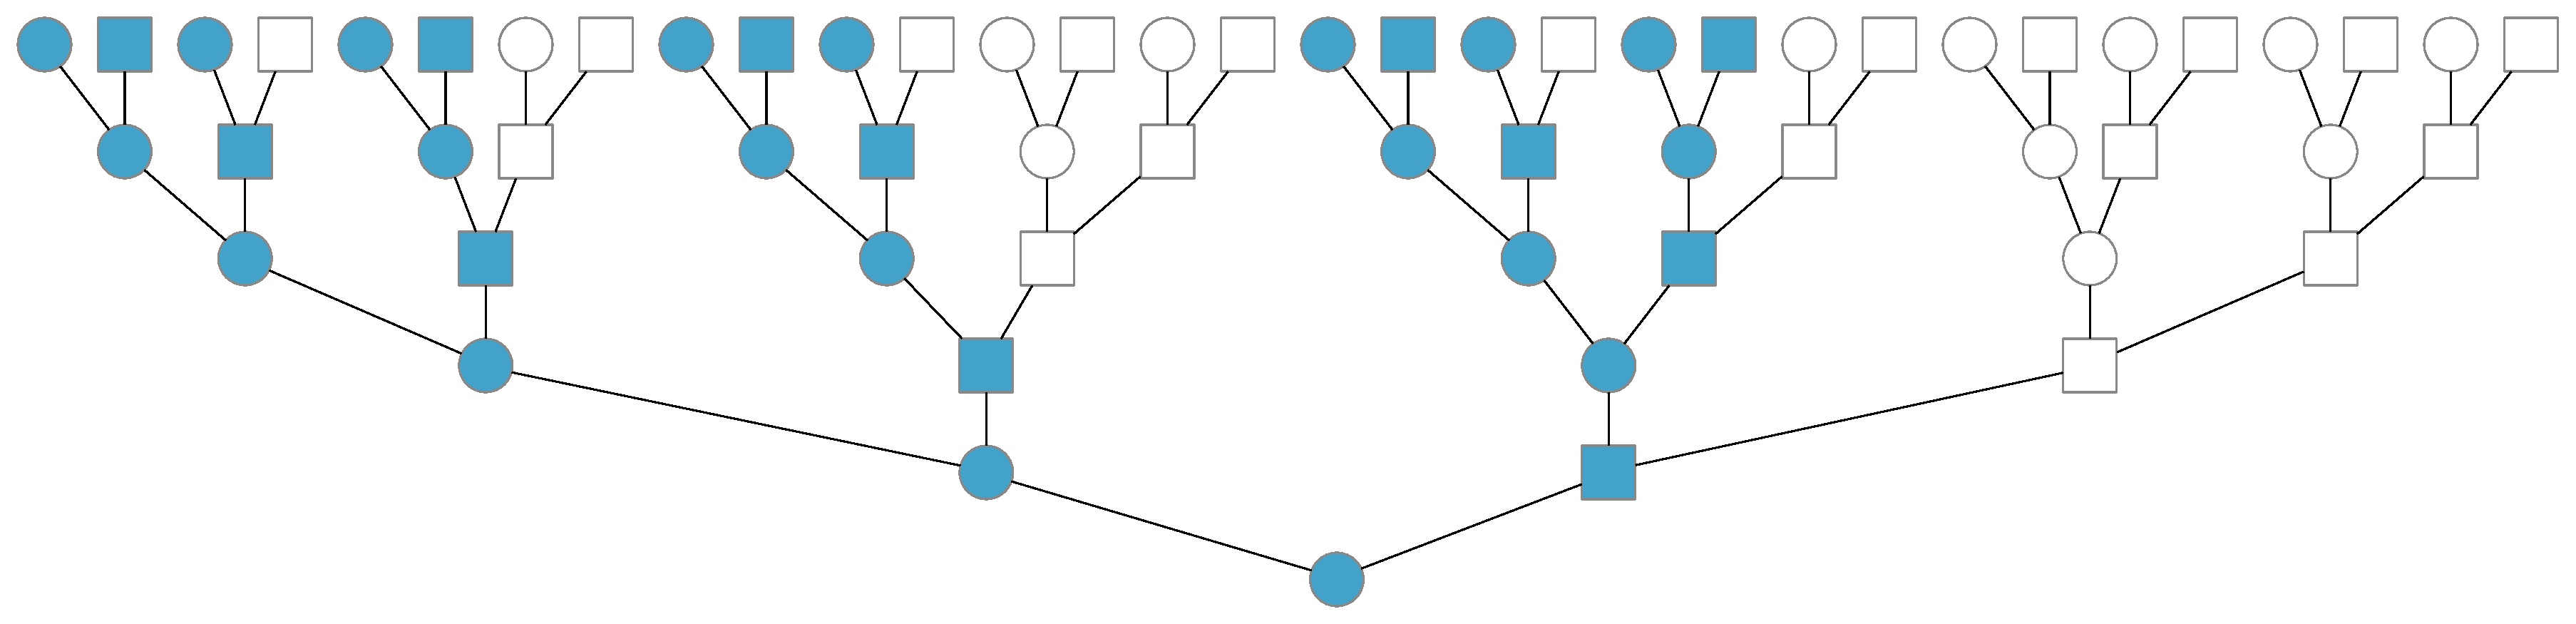
\includegraphics[width=\textwidth]{fig/x-genealogy}

  The X chromosome inheritance pattern:\\[1em]
  \begin{itemize}
    \item Every individual receives an X chromosome from his/her mother.
    \item Every female receives an X from her father (and sons do not receive an X from their fathers\footnote{We call this the \emph{no two adjacent male conditon}, as it means no two males are adjacent in an X genealogy}.).
  \end{itemize}
\end{frame}

\begin{frame}
  \frametitle{X Genealogies}
  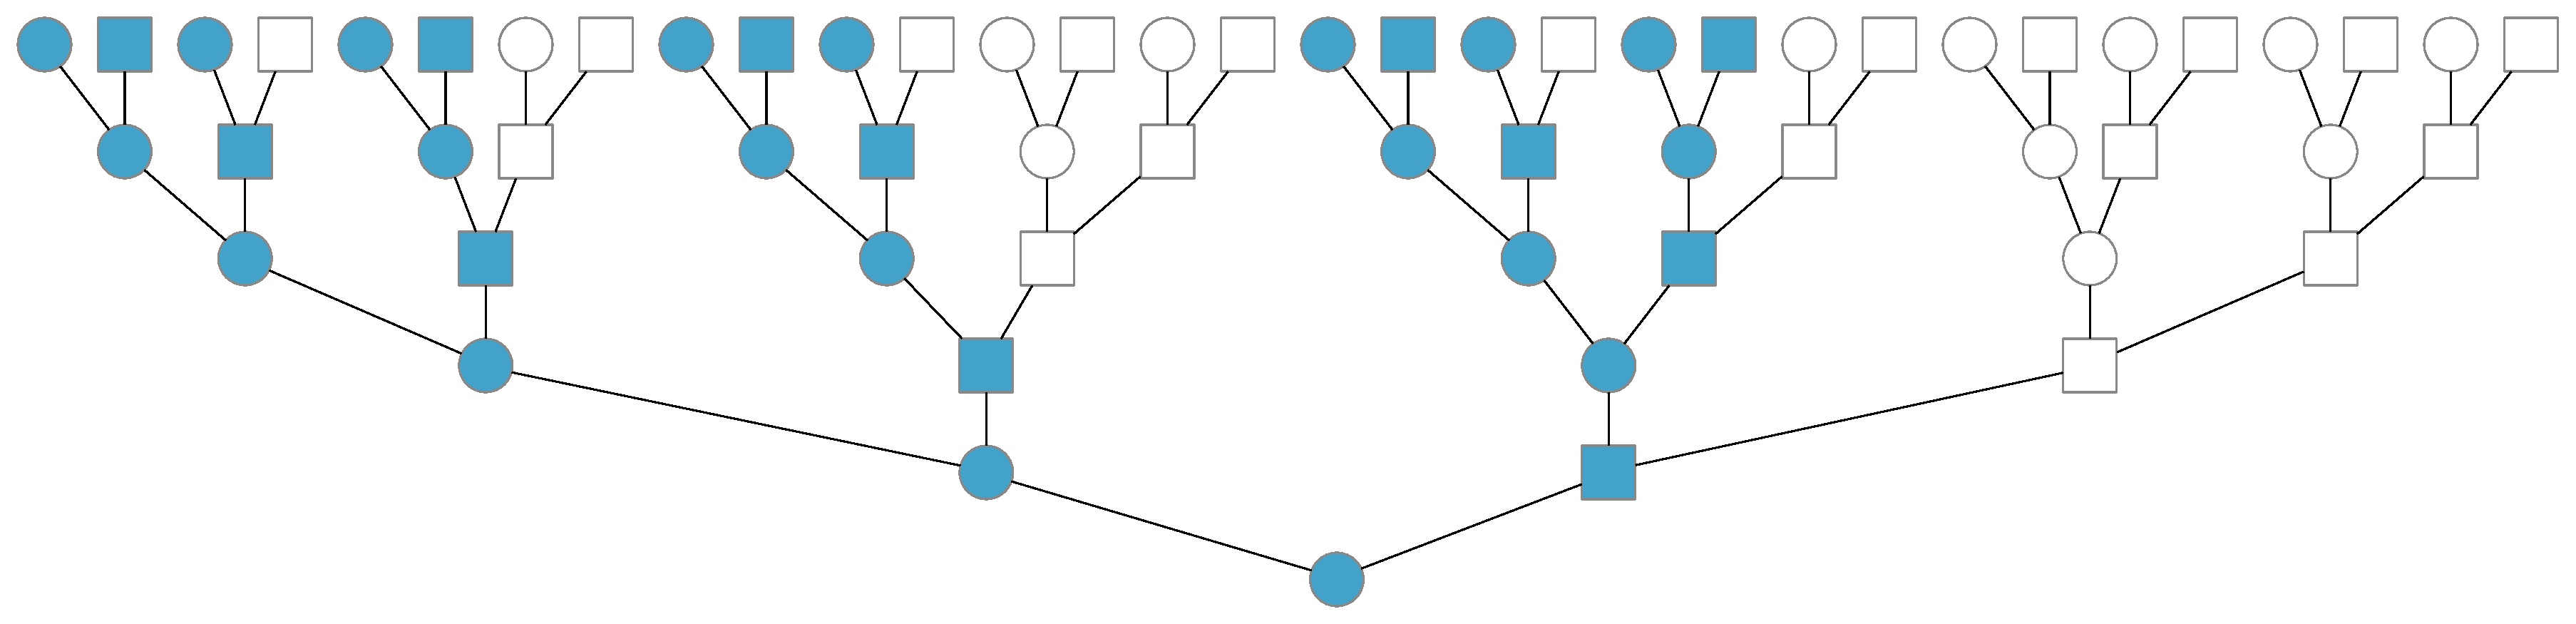
\includegraphics[width=\textwidth]{fig/x-genealogy}

  {\footnotesize Thus, a present-day female has 2, 3, 5, 8, 18, \ldots X
    ancestors.\\[1em]

  Encoding X inheritance rules as a set of recursion equations for the number
  of females ($f_k$), males ($m_k$), and total X ancestors $n_k = f_k + m_k$ for
  generation $k$ in the past:}

  \begin{align*}
    f_k &= n_{k-1} && \text{\footnotesize every individual receives an X chromosome from his/her mother}\\
    m_k &= f_{k-1} && \text{\footnotesize every female receives an X chromosome from her father}
  \end{align*}

\end{frame}


\begin{frame}
  \frametitle{X Genealogies}
  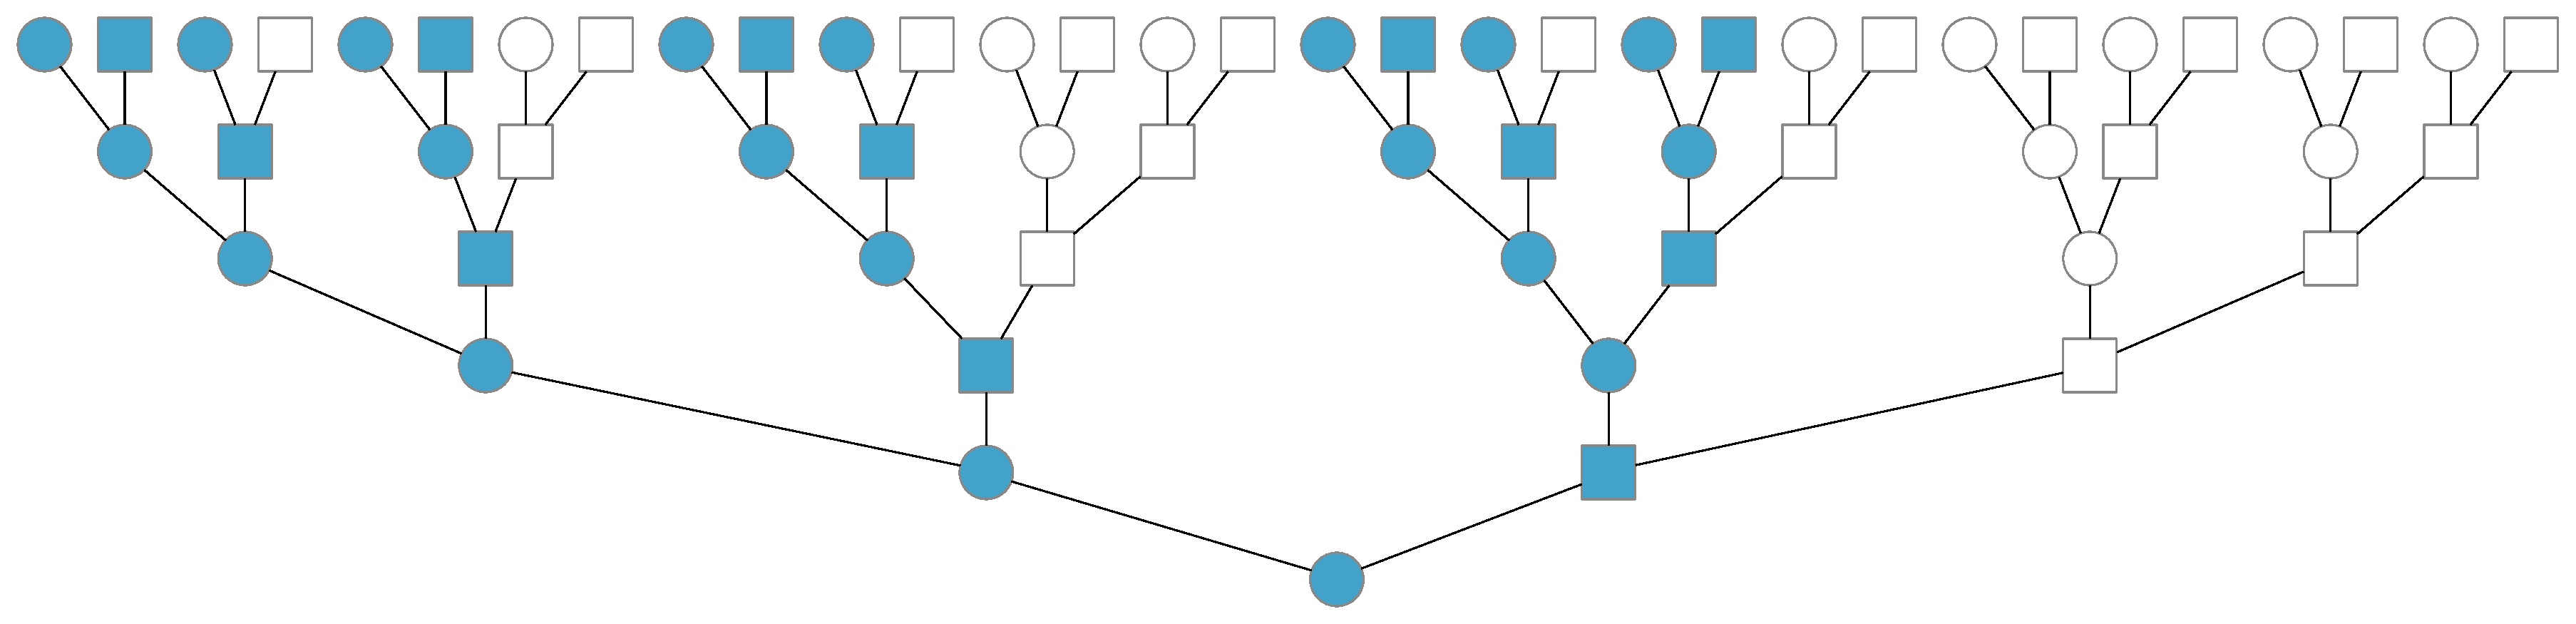
\includegraphics[width=\textwidth]{fig/x-genealogy}
  \begin{equation}
    n_k = n_{k-1} + n_{k-2}
  \end{equation}

  Which is the famous Fibonacci recurrence. Thus, $k$ generations back a present-day female has $\mathcal{F}_{k+2}$ X ancestors in her X chromosome genealogy.
\end{frame}

\begin{frame}
  \frametitle{The X Chromosome}
  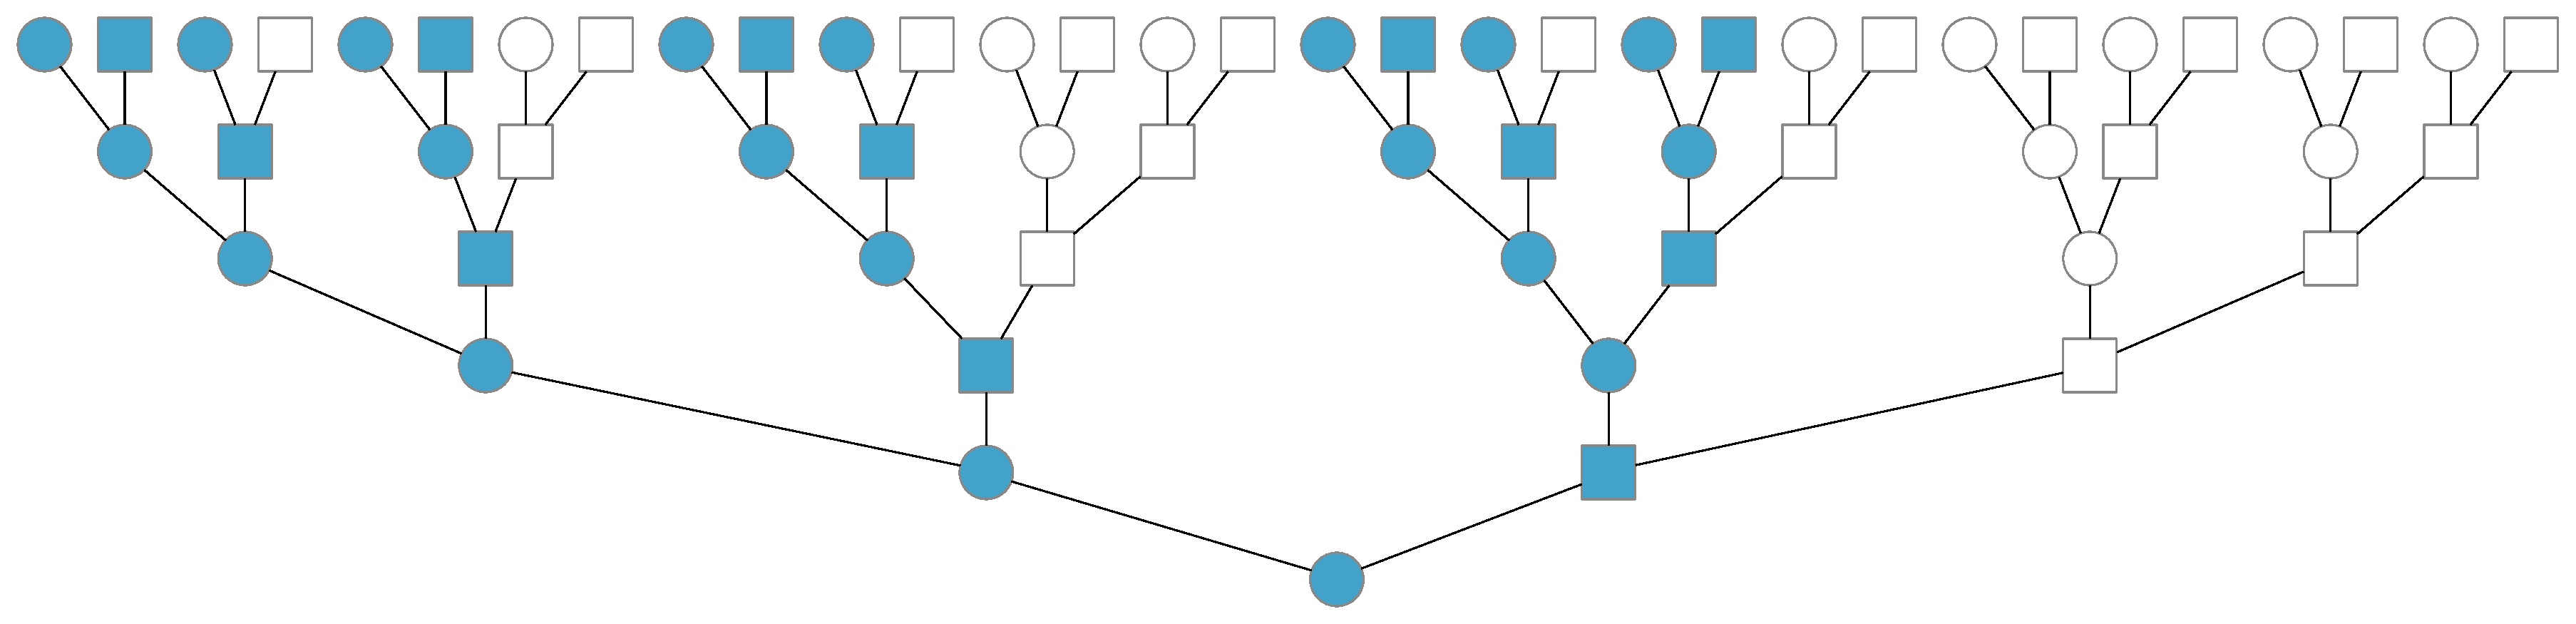
\includegraphics[width=\textwidth]{fig/x-genealogy}
   
\end{frame}




\begin{frame}
  \frametitle{}
  \begin{equation}
    \E[N] = \frac{1}{2^d} (\nu d + c)
  \end{equation}
\end{frame}


\begin{frame}
  \frametitle{Acknowledgments}
  \begin{columns}[c]
    \begin{column}{0.7\textwidth}
      Graham Coop\\
      Steve Mount\\[2em]
      Coop Lab
    \end{column} 
    \begin{column}{0.3\textwidth}
      
\includegraphics[width=0.6\textwidth]{fig/nsf}
    \end{column} 
  \end{columns} 
\end{frame}



\end{document}
